%%%%%%%%%%%%%%%%%%%%%%%%%%%%%%%%%%%%%%%%%
% Wenneker Article
% LaTeX Template
% Version 2.0 (28/2/17)
%
% This template was downloaded from:
% http://www.LaTeXTemplates.com
%
% Authors:
% Vel (vel@LaTeXTemplates.com)
% Frits Wenneker
%
% License:
% CC BY-NC-SA 3.0 (http://creativecommons.org/licenses/by-nc-sa/3.0/)
%
%%%%%%%%%%%%%%%%%%%%%%%%%%%%%%%%%%%%%%%%%

%----------------------------------------------------------------------------------------
%	PACKAGES AND OTHER DOCUMENT CONFIGURATIONS
%----------------------------------------------------------------------------------------

\documentclass[12pt, a4paper, twocolumn]{article} % 10pt font size (11 and 12 also possible), A4 paper (letterpaper for US letter) and two column layout (remove for one column)
\usepackage{setspace}
\usepackage{multirow}
\usepackage{float}
\usepackage{hyperref}
\usepackage[USenglish,UKenglish,french,spanish,italian]{babel}
\usepackage{graphicx}
\graphicspath{ {./Immagini/} }

%%%%%%%%%%%%%%%%%%%%%%%%%%%%%%%%%%%%%%%%%
% Wenneker Article
% Structure Specification File
% Version 1.0 (28/2/17)
%
% This file originates from:
% http://www.LaTeXTemplates.com
%
% Authors:
% Frits Wenneker
% Vel (vel@LaTeXTemplates.com)
%
% License:
% CC BY-NC-SA 3.0 (http://creativecommons.org/licenses/by-nc-sa/3.0/)
%
%%%%%%%%%%%%%%%%%%%%%%%%%%%%%%%%%%%%%%%%%

%----------------------------------------------------------------------------------------
%	PACKAGES AND OTHER DOCUMENT CONFIGURATIONS
%----------------------------------------------------------------------------------------

\usepackage[english]{babel} % English language hyphenation

\usepackage{microtype} % Better typography

\usepackage{amsmath,amsfonts,amsthm} % Math packages for equations

\usepackage[svgnames]{xcolor} % Enabling colors by their 'svgnames'

\usepackage[hang, small, labelfont=bf, up, textfont=it]{caption} % Custom captions under/above tables and figures

\usepackage{booktabs} % Horizontal rules in tables

\usepackage{lastpage} % Used to determine the number of pages in the document (for "Page X of Total")

\usepackage{graphicx} % Required for adding images

\usepackage{enumitem} % Required for customising lists
\setlist{noitemsep} % Remove spacing between bullet/numbered list elements

\usepackage{sectsty} % Enables custom section titles
\allsectionsfont{\usefont{OT1}{phv}{b}{n}} % Change the font of all section commands (Helvetica)

%----------------------------------------------------------------------------------------
%	MARGINS AND SPACING
%----------------------------------------------------------------------------------------

\usepackage{geometry} % Required for adjusting page dimensions

\geometry{
	top=1cm, % Top margin
	bottom=1.5cm, % Bottom margin
	left=2cm, % Left margin
	right=2cm, % Right margin
	includehead, % Include space for a header
	includefoot, % Include space for a footer
	%showframe, % Uncomment to show how the type block is set on the page
}

\setlength{\columnsep}{7mm} % Column separation width

%----------------------------------------------------------------------------------------
%	FONTS
%----------------------------------------------------------------------------------------

\usepackage[T1]{fontenc} % Output font encoding for international characters
\usepackage[utf8]{inputenc} % Required for inputting international characters

\usepackage{XCharter} % Use the XCharter font

%----------------------------------------------------------------------------------------
%	HEADERS AND FOOTERS
%----------------------------------------------------------------------------------------

\usepackage{fancyhdr} % Needed to define custom headers/footers
\pagestyle{fancy} % Enables the custom headers/footers

\renewcommand{\headrulewidth}{0.0pt} % No header rule
\renewcommand{\footrulewidth}{0.4pt} % Thin footer rule

\renewcommand{\sectionmark}[1]{\markboth{#1}{}} % Removes the section number from the header when \leftmark is used

%\nouppercase\leftmark % Add this to one of the lines below if you want a section title in the header/footer

% Headers
\lhead{} % Left header
\chead{\textit{\thetitle}} % Center header - currently printing the article title
\rhead{} % Right header

% Footers
\lfoot{} % Left footer
\cfoot{} % Center footer
\rfoot{\footnotesize Page \thepage\ of \pageref{LastPage}} % Right footer, "Page 1 of 2"

\fancypagestyle{firstpage}{ % Page style for the first page with the title
	\fancyhf{}
	\renewcommand{\footrulewidth}{0pt} % Suppress footer rule
}

%----------------------------------------------------------------------------------------
%	TITLE SECTION
%----------------------------------------------------------------------------------------

\newcommand{\authorstyle}[1]{{\large\usefont{OT1}{phv}{b}{n}\color{DarkRed}#1}} % Authors style (Helvetica)

\newcommand{\institution}[1]{{\footnotesize\usefont{OT1}{phv}{m}{sl}\color{Black}#1}} % Institutions style (Helvetica)

\usepackage{titling} % Allows custom title configuration

\newcommand{\HorRule}{\color{DarkGoldenrod}\rule{\linewidth}{1pt}} % Defines the gold horizontal rule around the title

\pretitle{
	\vspace{-30pt} % Move the entire title section up
	\HorRule\vspace{10pt} % Horizontal rule before the title
	\fontsize{25}{40}\usefont{OT1}{phv}{b}{n}\selectfont % Helvetica
	\color{DarkRed} % Text colour for the title and author(s)
}

\posttitle{\par\vskip 15pt} % Whitespace under the title

\preauthor{} % Anything that will appear before \author is printed

\postauthor{ % Anything that will appear after \author is printed
	\vspace{10pt} % Space before the rule
	\par\HorRule % Horizontal rule after the title
	\vspace{20pt} % Space after the title section
}

%----------------------------------------------------------------------------------------
%	ABSTRACT
%----------------------------------------------------------------------------------------

\usepackage{lettrine} % Package to accentuate the first letter of the text (lettrine)
\usepackage{fix-cm}	% Fixes the height of the lettrine

\newcommand{\initial}[1]{ % Defines the command and style for the lettrine
	\lettrine[lines=3,findent=4pt,nindent=0pt]{% Lettrine takes up 3 lines, the text to the right of it is indented 4pt and further indenting of lines 2+ is stopped
		\color{DarkGoldenrod}% Lettrine colour
		{#1}% The letter
	}{}%
}

\usepackage{xstring} % Required for string manipulation

\newcommand{\lettrineabstract}[1]{
	\StrLeft{#1}{1}[\firstletter] % Capture the first letter of the abstract for the lettrine
	\initial{\firstletter}\textbf{\StrGobbleLeft{#1}{1}} % Print the abstract with the first letter as a lettrine and the rest in bold
}

%----------------------------------------------------------------------------------------
%	BIBLIOGRAPHY
%----------------------------------------------------------------------------------------

\usepackage{biblatex} %Imports biblatex package
\addbibresource{sample.bib} %Import the bibliography file

\usepackage[autostyle=true]{csquotes} % Required to generate language-dependent quotes in the bibliography

\addto\captionsenglish{\renewcommand*\contentsname{Indice} } % Specifies the document structure and loads requires packages

%----------------------------------------------------------------------------------------
%	ARTICLE INFORMATION
%----------------------------------------------------------------------------------------

\title{Data Science Lab: Vendite E-commerce} % The article title

\author{
    Ruben Agazzi 844736\\
	Fabrizio Cominetti 882737\\
	Davide Abete x\\
	Tommaso Strada x\\
	Alessandro Fasani x % Authors
}

%----------------------------------------------------------------------------------------

\begin{document}

\selectlanguage{italian}

% \maketitle % Print the title

\thispagestyle{firstpage} % Apply the page style for the first page (no headers and footers)

%----------------------------------------------------------------------------------------
%	ABSTRACT
%----------------------------------------------------------------------------------------
\twocolumn[
  \begin{@twocolumnfalse}
    \maketitle
    \begin{abstract}
      \noindent{L'obiettivo principale del progetto è quello di valutare e selezionare il miglior modello predittivo relativamente alle stime delle vendite di alcuni settori, precisamente Pesca, Calcio e Casual, di un attività di e-commerce.}\\
      Il periodo preso in considerazione va dal giorno 01-01-2014 al giorno 31-12-2021.\\
      Per un attività commerciale presente sulla rete è di fondamentale importanza prevedere le vendite che saranno effettuate nei periodi successivi per ogni settore a disposizione, in modo tale da organizzare disponibilità di magazzino e di spedizione.\\
      I dati sono stati modellati in funzione dell'obiettivo e aggregati secondo diverse granularità, ovvero con frequenza annuale, trimestrale, e settimanale, in modo tale da valutare le performance dei modelli presi in considerazione.\\
      Come sarà possibile verificare nel proseguio del report, la granularità più efficace, relativamente agli obiettivi preposti dal progetto, è risultata quella x.\\
      Il progetto è stato effettuato prendendo in considerazione i tre settori con maggiore disponibilità effettiva di osservazioni, ma i modelli utilizzati possono essere applicati anche ad altri settori, per realizzare in questo modo una panoramica completo sull'intero e-commerce.
    \end{abstract}
  \end{@twocolumnfalse}]

\bigskip

\clearpage
% \lettrineabstract{x}
\bigskip
\tableofcontents

%----------------------------------------------------------------------------------------
%	ARTICLE CONTENTS
%----------------------------------------------------------------------------------------

\section{Introduzione}
La realizzazione di questo progetto ha visto come obiettivo principale quello di testare, valutare e decretare il miglior modello predittivo al fine di stimare le vendite in euro realizzate dai vari settori all'interno di un e-commerce.\\
Prima di tutto, i dati sono stati pre-processati e 'puliti', in modo tale da renderli efficaci e ottimali rispetto allo scopo del progetto. I modelli predittivi, infatti, richiedevano un certo tipo di modellazione dei dati in input per utilizzarli al proprio interno e produrre delle previsioni.\\
Una volta effettuato il pre-processing dei dati, il focus è passato sul test dei vari modelli, ognuno con le diverse granularità scelte in fase di programmazione.\\
Lorem ipsum dolor sit amet %(vedi report esempio)\\
Periodo scelto e caratteristiche periodo temporale.

\subsection{Punti Principali}
\begin{itemize}
	\item Vendite 
	\item Settori 
	\item Previsione
\end{itemize}

\subsection*{Heading on level 2}
Lorem ipsum dolor sit amet, consectetuer adipiscing elit. Aenean commodo ligula eget dolor. Aenean massa. Cum sociis natoque penatibus et magnis dis parturient montes, nascetur ridiculus mus. Donec quam felis, ultricies nec, pellentesque eu, pretium quis, sem.
\bigskip

\begin{itemize}
	\item First item in a list 
	\item Second item in a list 
	\item Third item in a list
\end{itemize}
Lorem ipsum dolor sit amet, consectetuer adipiscing elit. Aenean commodo ligula eget dolor. Aenean massa. Cum sociis natoque penatibus et magnis dis parturient montes, nascetur ridiculus mus. Donec quam felis, ultricies nec, pellentesque eu, pretium quis, sem. Nulla consequat massa quis enim. 

Donec pede justo, fringilla vel, aliquet nec, vulputate eget, arcu. In enim justo, rhoncus ut, imperdiet a, venenatis vitae, justo. Nullam dictum felis eu pede mollis pretium. Integer tincidunt. Cras dapibus. Vivamus elementum semper nisi. Aenean vulputate eleifend tellus. Aenean leo ligula, porttitor eu, consequat vitae, eleifend ac, enim. Aliquam lorem ante, dapibus in, viverra quis, feugiat a, tellus. Phasellus viverra nulla ut metus varius laoreet. Quisque rutrum. Aenean imperdiet. Etiam ultricies nisi vel augue. Curabitur ullamcorper ultricies 

\section{Obiettivo}
L'obiettivo del progetto è quello di identificare il miglior modello predittivo da fornire ai gestori dell'e-commerce in questione.\\
Conoscere la previsione relativa agli incassi (in euro) dei vari settori all'interno del sito potrebbe infatti essere utile a diversi scopi all'interno dell'azienda, come ad esempio in fase di programmazione e ordini di materiale, ma anche per avere un'idea di quando applicare o meno determinati sconti e promozioni ai vari settori, con il fine di raggiungere gli obiettivi di vendita prefissati.\\
Periodo\\
Realizzazione di dashboard\\
Destinatari del progetto.

\section{Aspetti Metodologici}
I modelli selezionati ed utilizzati all'interno del progetto sono i seguenti: ARIMA, TBATS, PROPHET, XGBOOST.\\
Di seguito osserviamo i modelli in modo più approfondito da un punto di vista teorico.

\subsection{ARIMA}
In statistica per modello ARIMA (acronimo di AutoRegressive Integrated Moving Average) si intende una particolare tipologia di modelli atti ad indagare serie storiche che presentano caratteristiche particolari. Fa parte della famiglia dei processi lineari non stazionari.\\
Un modello ARIMA(p,d,q) deriva da un modello ARMA(p,q) a cui sono state applicate le differenze di ordine d per renderlo stazionario. In caso di stagionalità nei dati si parla di modelli SARIMA o ARIMA(p,d,q)(P,D,Q).\\
Dunque, il modello ARIMA nasce aggiungendo l'integrazione (I) alla combinazione dei modelli autoregressivo (AR) e a media mobile (MA). Il modello ARIMA è composto dalle seguenti componenti:
\begin{description}
	\item[P] l'ordine della componente autoregressiva
	\item[D] grado della differenziazione
	\item[Q] ordine della componente a media mobile
\end{description}
Siccome, appunto, un modello ARIMA integra la componente autoregressiva e di media mobile di una serie storica, può essere così definito:
\[
(1 - \sum_{i=1}^{p'}\alpha_iL^i)X_t = (1+\sum_{i=1}^{q}\theta_iL^i)	
\]
 Un modello integrato ARMA di ordine d è un processo stocastico che diventa stazionario dopo essere differenziato d volte.\\

Abbiamo creato 12 diversi modelli, in modo da predire i valori settimanali, mensili, trimestrali e annuali dei 3 settori di vendita selezionati, ovver calcio, pesca e casual. I parametri dei modelli ARIMA e SARIMA sono trovati minimizzando l'AIC.

I modelli ottenuti e i loro parametri sono i seguenti:
\begin{itemize}
	\item Annuale pesca: ARIMA model (0,1,0)(0,0,0)
	\item Trimestrale pesca: ARIMA model (0,2,1)(0,0,0)
	\item Mensile pesca: SARIMA model (0,1,1)(1,0,0)
	\item Settimanale pesca: SARIMA model (2,1,2)(1,0,0)
	\item Annuale calcio: ARIMA model (0,1,0)(0,0,0)
	\item Trimestrale calcio: SARIMA model (0,0,1)(1,1,0)
	\item Mensile calcio: SARIMA model (0,0,1)(0,1,0)
	\item Settimanale calcio: SARIMA model (1,0,0)(1,0,0)
	\item Annuale casual: ARIMA model (0,1,0)(0,0,0)
	\item Trimestrale casual: SARIMA model (1,1,0)(1,0,0)
	\item Mensile casual: SARIMA model (1,1,3)(1,0,0)
	\item Settimanale casual: ARIMA model (1,0,0)(0,0,0)
\end{itemize}

\subsection{TBATS}
Il modello TBATS è in grado di considerare e lavorare con stagionalità multiple e complesse.\\
TBATS è l'acronimo di Trigonometric seasonality, Box-Cox transformation, ARMA errors, Trend and Seasonal components.\\
In questo modello, ogni stagionalità è modellata su di una rappresentazione trigonometrica, basata sulla serie di Fourier. Uno dei principali vantaggi di questo approccio è che richiede solo due 'seed', indipendentemente dalla lunghezza del periodo. Un altro vantaggio è la possibilità di modellare effetti stagionali di lunghezza non intera. Ad esempio, data una serie di osservazioni giornaliere, è possibile modellare gli anni bisestili con una stagione di lunghezza 365,25.\\
Il modello TBATS prende in considerazione varie alternative ed è in grado di adattarsi a diversi modelli. Prenderà in considerazione modelli con le seguenti caratteristiche:
\begin{itemize}
\item con e senza trasformazione Box-Cox
\item con e senza Trend
\item con e senza smorzamento del trend
\item con e senza processo ARMA(p,q) utilizzato per modellare i residui
\item modello non stagionale
\item varie quantità di armoniche utilizzate per modellare gli effetti stagionali
\end{itemize}
Il modello finale sarà poi scelto utilizzando il criterio di informazione di Akaike (AIC).\\
Nella figura sottostante possiamo osservare due formulazioni matematiche del modello in questione.

\begin{figure}
  \caption{Dispensa}
  \begin{center}
    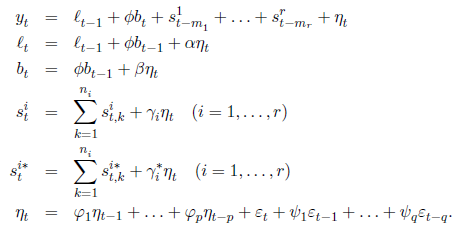
\includegraphics{tbats.png}
  \end{center}
\end{figure}

\begin{figure}
  \caption{\protect\cite{tbats}}
  \begin{center}
    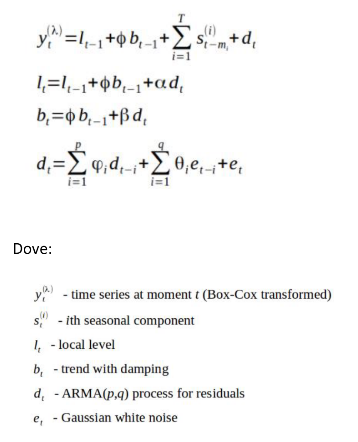
\includegraphics{tbats2.png}
  \end{center}
\end{figure}

\subsection{PROPHET}
Prophet è un modello dedito alla previsione di serie storiche basata su modelli additivi, dove i trend non lineari sono analizzati con diverse stagionalità. Il modello decompone la serie storica in trend, stagionalità ed effetti di festività. 
\begin{description}
	\item[First] This is the first item
	\item[Last] This is the last item
\end{description}
Può essere quindi considerato un modello di regressione non lineare, della forma:
\\
$y(t) = g(t) + s(t) + h(t) + e(t)$
\\
dove:
\begin{description}
	\item[g(t)] descrive una tendenza a tratti lineare delle variazioni non periodiche nei dati delle serie temporali (o termine di crescita)
	\item[s(t)] indica i vari modelli stagionali generati dai cambiamenti periodici come la stagionalità giornaliera, settimanale o annuale
	\item[h(t)] rappresenta gli effetti festivi che si possono verificare su cadenze irregolari, ad esempio su un giorno o su un periodo di più giorni
	\item[e(t)] sono termini di errore, ciò che non viene spiegato dal modello
\end{description}
\cite{mathprophet}\cite{fbprophet}
\\
In altri termini l’equazione può essere così scritta:
\begin{figure}
  \caption{}
  \begin{center}
    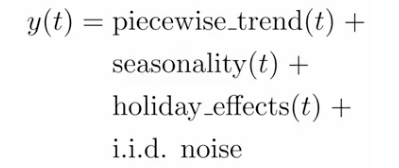
\includegraphics[width=75mm,scale=0.5]{prophet.png}
  \end{center}
\end{figure}
\\
Il modello Prophet prevede due possibili modelli di tendenze per la componente g(t), un modello di crescita saturante e un modello lineare a tratti. La componente stagionale s(t) fornisce adattabilità al modello consentendo periodiche modifiche basate su cambiamenti della stagionalità infragiornaliere, giornaliere, settimanali e annuali. Questa componente per impostazione predefinita, prevede l'utilizzo dell’ordine 10 per la stagionalità annuale e l'ordine 3 per quella settimanale. La componente h(t) considera eventi prevedibili dell'anno, ad esempio  il Venerdì nero, il Superbowl o Natale. Per utilizzare questa funzione, l'utente deve fornire un elenco personalizzato di eventi festivi e l’incorporazione di questa lista nel modello è fatta supponendo che gli effetti delle vacanze siano indipendenti. Il modello viene stimato utilizzando un approccio bayesiano per consentire la selezione automatica dei change points e di altri parametri del modello, se non esplicitamente specificati. Date le sue caratteristiche performa meglio con le serie temporali che hanno forti effetti stagionali e numerose stagioni di dati storici. Il modello è caratterizzato da diversi vantaggi: è preciso e veloce, per questo viene utilizzato ad esempio in molte applicazioni su Facebook per produrre previsioni affidabili per la pianificazione e la definizione degli obiettivi, completamente automatico, in quanto fornisce una previsione ragionevole su dati disordinati senza sforzo manuale, genera previsioni adattabili fornendo molte possibilità agli utenti di modificare e regolare le previsioni al fine di migliorarle, gestisce bene le variazioni stagionali, ed infine, è robusto nei confronti dei valori anomali e resiliente ai dati mancanti.\\

\subsection{XGBOOST}
XGBoost is an efficient implementation of gradient boosting for classification and regression problems.\\
XGBoost can also be used for time series forecasting, although it requires that the time series dataset be transformed into a supervised learning problem first. It also requires the use of a specialized technique for evaluating the model called walk-forward validation, as evaluating the model using k-fold cross validation would result in optimistically biased results.\\
\\
XGBRegressor uses a number of gradient boosted trees (referred to as n\_estimators in the model) to predict the value of a dependent variable. This is done through combining decision trees (which individually are weak learners) to form a combined strong learner.\\
When forecasting a time series, the model uses what is known as a lookback period to forecast for a number of steps forward. For instance, if a lookback period of 1 is used, then the X\_train (or independent variable) uses lagged values of the time series regressed against the time series at time t (Y\_train) in order to forecast future values.\\
\cite{xgboost}

\begin{description}
	\item[First] This is the first item
	\item[Last] This is the last item
\end{description}
Nullam dictum felis eu pede mollis pretium. Integer tincidunt. Cras dapibus. Vivamus elementum semper nisi. Aenean vulputate eleifend tellus. Aenean leo ligula, porttitor eu, consequat vitae, eleifend ac, enim. Aliquam lorem ante, dapibus in, viverra quis, feugiat a, tellus. Phasellus viverra nulla ut metus varius laoreet. Quisque rutrum. Aenean imperdiet. Etiam ultricies nisi vel augue. Curabitur ullamcorper ultricies

\section{Dati}
Il dataset utilizzato per il progetto è il dataset "serie-storiche-ecommerce" ed è un file di tipo CSV (Comma Separated Values).\\
Il file si presentava con un problema relativo alla divisione dell'importo in euro in due differenti colonne, è stata perciò effettuata una correzione per unire le due colonne citate in un unica colonna.\\
Considerando la correzione effettuata, all'interno del file sono presenti le seguenti colonne:
\begin{description}
	\item[data] contenente la data di rilevazione nel seguente formato: DD/MM/YYYY
	\item[totale] importo in euro dell'incasso di uno specifico settore in quel giorno
	\item[settore] testo che identifica il settore dell'e-commerce di riferimento
\end{description}
Per ciascun settore è dunque presente il totale delle vendite (in euro) effettuate in quella data. Le rilevazioni sono dunque giornaliere e divise per settore. Sono pochi i settori che presentano una fetta consistente di rilevazioni, al contrario, per molti settori il numero di osservazioni è limitato.\\
% magari aggiungere immagini relative a numero di osservazioni dei settori
Per questo motivo le analisi successive saranno effettuate considerando i settori con il maggior numero di osservazioni presenti.\\
I dati a disposizione coprono il periodo compreso tra il 2 febbraio 2013 e l'8 aprile 2022.\\
Il file iniziale è composto da un totale di 25262 righe e dalle 3 colonne descritte sopra.

\subsection{Manipolazione Dati}
Durante la fase iniziale di esplorazione dei dati, abbiamo notato la presenza di molti valori mancanti all'interno del dataset; in particolare la maggior parte di questi valori appartenevano all'anno 2013. In questo caso abbiamo deciso di rimuovere completamente l'anno in questione in modo da avere dati continui sugli anni precedenti, evitando di allenare i modelli su dati frammentati e incompleti.
\subsection{Aggreazione dei dati}
Una volta rimossi i valori precedenti abbiamo raggruppato i dati per i 3 settori di vendita scelti, ovvero pesca, calcio e casual. In seguito i vari dataset già raggruppati per settori sono stati ulteriormente raggruppati in base a diversi periodi di tempo, in modo da avere una granularità dei dati più varia. In particolare sono stati creati dataset relativi alle vendite settimanali, mensili, trimestrali e annuali.
\section{Analisi per settore}
Ora seguirà una breve analisi dei risultati, divisa per settore di vendita, in particolare indicheremo il modello migliore ottenuto per lo specifico settore di vendita. In seguito presenteremo i risultati completi
\subsection{Analisi Pesca}
Nel contesto degli algoritmi usati per il settore di vendita "Pesca", al netto dei raggruppamenti, il modello che ha avuto risultati migliori è "modello", in particolare applicato su un raggruppamento "raggruppamento" dei dati. Il modello in questione ha avuto un MAPE(Mean Absolute Percentage Error) pari a "perc".
\begin{figure}
  \caption{}
  \begin{center}
    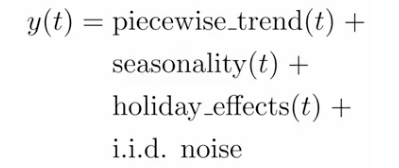
\includegraphics[width=75mm,scale=0.5]{prophet.png}
  \end{center}
\end{figure}

\subsection{Analisi Calcio}
Per quanto riguarda ai dati relativi al settore di vendita "Calcio", il modello migliore che trovato è stato "modello" con un Mean Percentage Error pari a "perc". Questo modello inoltre è stato applicato ai dati raggruppati "raggruppamento"
\begin{figure}
  \caption{}
  \begin{center}
    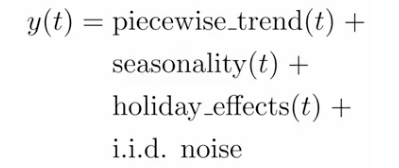
\includegraphics[width=75mm,scale=0.5]{prophet.png}
  \end{center}
\end{figure}
\subsection{Analisi Casual}
Infine, per quanto riguarda il settore di vendite Casual, il modello che ha ottenuto risultati migliori è "modello" applicato ai dati raggruppati "raggruppanto". Il MAPE ottenuto da questo modello è pari a "perc"
\begin{figure}
  \caption{}
  \begin{center}
    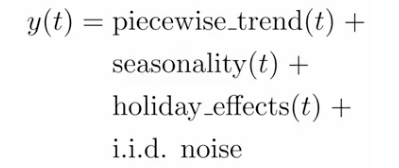
\includegraphics[width=75mm,scale=0.5]{prophet.png}
  \end{center}
\end{figure}

\section{Risultati}
Al fine di valutare e selezionare il modello più indicato e preciso relativamente alle finalità del progetto, si è scelto di utilizzare una metrica, 'MAPE', in grado di tener conto anche dell'errore di previsione.\\
Di seguito il MAPE (Mean Absolute Percentage Error), o errore percentuale medio assoluto, dal punto di vista teorico:\\
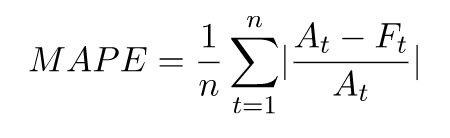
\includegraphics[width=75mm,scale=0.5]{mape.png}
\\
dove:
\begin{description}
	\item[$A_t$] sono i valori reali
	\item[$F_t$] sono i valori predetti
	\item[n] rappresenta il numero di osservazioni
\end{description}

La metrica MAPE consiste nella media aritmetica dei rapporti tra il valore assoluto degli errori di previsione e la domanda che si è effettivamente verificata.\\
Illustriamo di seguito i valori della metrica considerata per ciascuno dei modelli testati.

\begin{table}[H]
\caption{MAPE dati annuali}
\centering
	\begin{tabular}{lllr}
		\toprule
		\multicolumn{4}{c}{MAPE} \\
		\cmidrule(r){2-4}
			Modello & Pesca & Calcio & Casual \\
		\midrule
			ARIMA & 31.75\% & 28.5\% & 31.74\% \\
			TBATS & 28.6\% & 50.08\% & 28.32\% \\
			PROPHET & 36.88\% & 97.64\% & 36.88\% \\
			XGBOOST & X\% & X\% & X\% \\
		\bottomrule
	\end{tabular}
\end{table}

\begin{table}[H]
	\caption{MAPE dati trimestrali}
	\centering
		\begin{tabular}{lllr}
			\toprule
			\multicolumn{4}{c}{MAPE} \\
			\cmidrule(r){2-4}
				Modello & Pesca & Calcio & Casual \\
			\midrule
				ARIMA & 28.67\% & 80.68\% & 73.66\% \\
				TBATS & 42.16\% & 39.5\% & 37.35\% \\
				PROPHET & 45.87\% & 86.19\% & 63.67\% \\
				XGBOOST & X\% & X\% & X\% \\
			\bottomrule
		\end{tabular}
	\end{table}

	\begin{table}[H]
		\caption{MAPE dati mensili}
		\centering
			\begin{tabular}{lllr}
				\toprule
				\multicolumn{4}{c}{MAPE} \\
				\cmidrule(r){2-4}
					Modello & Pesca & Calcio & Casual \\
				\midrule
					ARIMA & 33.60\% & 116.59\% &234.71\% \\
					TBATS & 47.09\% & 58.05\% & 33.92\% \\
					PROPHET & 12.86\% & 106.61\% & 22.88\% \\
					XGBOOST & X\% & X\% & X\% \\
				\bottomrule
			\end{tabular}
		\end{table}
		
		\begin{table}[H]
			\caption{MAPE dati settimanali}
			\centering
				\begin{tabular}{lllr}
					\toprule
					\multicolumn{4}{c}{MAPE} \\
					\cmidrule(r){2-4}
						Modello & Pesca & Calcio & Casual \\
					\midrule
						ARIMA & 71.09\% & 111.99\% & 118.32\% \\
						TBATS & 40.63\% & 159.13\% & 41.63\% \\
						PROPHET & 18.97\% & 19.07\% & 57.51\% \\
						XGBOOST & X\% & X\% & X\% \\
					\bottomrule
				\end{tabular}
			\end{table}


\section{Conclusioni}
In conclusione abbiamo notato che il modello più performante ottenuto è "modello" applicato ai dati del settore "settore" raggruppati "raggruppamento". D'altro canto il modello che ha avuto la peggiore performance è il modello SARIMA applicato al settore casual con raggruppamento dei dati mensile. Alcuni ulteriori sviluppi potrebbero consistere nel test di altri algoritmi per la previsione di serie storiche, magari utilizzando anche tecniche di deep learning.

\begin{align}
	A = 
	\begin{bmatrix}
	A_{11} & A_{21} \\
  	A_{21} & A_{22}
	\end{bmatrix}
\end{align}

\nocite{*} %aggiunge a bibliografia gli elementi non citati nel testo
\printbibliography[title={Bibliografia}] %Prints bibliography

\end{document}
